% This is the Reed College LaTeX thesis template. Most of the work
% for the document class was done by Sam Noble (SN), as well as this
% template. Later comments etc. by Ben Salzberg (BTS). Additional
% restructuring and APA support by Jess Youngberg (JY).
% Your comments and suggestions are more than welcome; please email
% them to cus@reed.edu
%
% See http://web.reed.edu/cis/help/latex.html for help. There are a
% great bunch of help pages there, with notes on
% getting started, bibtex, etc. Go there and read it if you're not
% already familiar with LaTeX.
%
% Any line that starts with a percent symbol is a comment.
% They won't show up in the document, and are useful for notes
% to yourself and explaining commands.
% Commenting also removes a line from the document;
% very handy for troubleshooting problems. -BTS

% As far as I know, this follows the requirements laid out in
% the 2002-2003 Senior Handbook. Ask a librarian to check the
% document before binding. -SN

%%
%% Preamble
%%
% \documentclass{<something>} must begin each LaTeX document
\documentclass[12pt,twoside]{reedthesis}
% Packages are extensions to the basic LaTeX functions. Whatever you
% want to typeset, there is probably a package out there for it.
% Chemistry (chemtex), screenplays, you name it.
% Check out CTAN to see: http://www.ctan.org/
%%
\usepackage{graphicx,latexsym}
\usepackage{amsmath}
\usepackage{amssymb,amsthm}
\usepackage{longtable,booktabs,setspace}
\usepackage{chemarr} %% Useful for one reaction arrow, useless if you're not a chem major
\usepackage[hyphens]{url}
% Added by CII
\usepackage[hidelinks]{hyperref}
\usepackage{lmodern}
\usepackage{float}
\floatplacement{figure}{H}
% End of CII addition
\usepackage{rotating}

% Next line commented out by CII
%%% \usepackage{natbib}
% Comment out the natbib line above and uncomment the following two lines to use the new
% biblatex-chicago style, for Chicago A. Also make some changes at the end where the
% bibliography is included.
%\usepackage{biblatex-chicago}
%\bibliography{thesis}


% Added by CII (Thanks, Hadley!)
% Use ref for internal links
\renewcommand{\hyperref}[2][???]{\autoref{#1}}
\def\chapterautorefname{Chapter}
\def\sectionautorefname{Section}
\def\subsectionautorefname{Subsection}
% End of CII addition

% Added by CII
\usepackage{caption}
\captionsetup{width=5in}
% End of CII addition

% \usepackage{times} % other fonts are available like times, bookman, charter, palatino


% To pass between YAML and LaTeX the dollar signs are added by CII
\title{\textbf{\Huge{Numerical methods for the \\[20pt] Heston model}}}
\author{Fernando O. Teixeira}
% The month and year that you submit your FINAL draft TO THE LIBRARY (May or December)
\date{setembro 19, 2017}
\division{Applied Mathematics}
\advisor{Hugo Alexander de la Cruz Cancino}
%If you have two advisors for some reason, you can use the following
% Uncommented out by CII
% End of CII addition

%%% Remember to use the correct department!
\department{Mathematics}
% if you're writing a thesis in an interdisciplinary major,
% uncomment the line below and change the text as appropriate.
% check the Senior Handbook if unsure.
%\thedivisionof{The Established Interdisciplinary Committee for}
% if you want the approval page to say "Approved for the Committee",
% uncomment the next line
%\approvedforthe{Committee}

% Added by CII
%%% Copied from knitr
%% maxwidth is the original width if it's less than linewidth
%% otherwise use linewidth (to make sure the graphics do not exceed the margin)
\makeatletter
\def\maxwidth{ %
  \ifdim\Gin@nat@width>\linewidth
    \linewidth
  \else
    \Gin@nat@width
  \fi
}
\makeatother

\renewcommand{\contentsname}{Table of Contents}
% End of CII addition

\setlength{\parskip}{0pt}

% Added by CII

\providecommand{\tightlist}{%
  \setlength{\itemsep}{0pt}\setlength{\parskip}{0pt}}

\Acknowledgements{
\textbf{\\ \\ \\ \\ \\ \\ \\ \\ \\ \\ \\ \\ \\ \\ \\ \\ \\ \\ \\ \\ \\ \\ \\ \\ \\ \\ \\ \\ \\ \\ \\ \\ \\ \\ \\ \\ \\ \\ \\ \\ \\ \\ \\ \\ \\ \\ \\ \\ \\ \\ \\ \\ \\ \\ \\ \\ \\ \\ \\ \\ \\ \\ \\ }
You get pseudo-order when you seek order; you only get a measure of
order and control when you embrace randomness. --- Nassim Nicholas Taleb
}

\Dedication{

}

\Preface{

}

\Abstract{
In this thesis we revisit some of the numerical methods for solving the
Heston model's European call. Specifically, we approach Euler's, the
Kahl-Jackel an two versions of the exact algorithm schemes. To perform
this task, firstly we present a literature review which brings
stochastic calculus, the Black-Scholes (BS) model and its limitations,
the stochastic volatility methods and why they resolve the issues of the
BS model, and the peculiarities of the numerical methods - convergence,
discretization and stability. Since it is impossible to have a deep
approach to all these topics, we provide recommendations when we
acknowledge that the reader might need more specifics. We introduce the
methods previously cited providing all our implementations in R
language. Also, we deliver an R package with these functions and others.
\newline \newline \textbf{Keywords:} Heston, Stochastic, Volatility,
Black-Scholes, European call, R
}

	\usepackage{mathtools}
	\usepackage{cancel}
	\graphicspath{ {figure/} }
	\usepackage{enumitem}
	\usepackage{caption}
	\usepackage{graphicx}
% End of CII addition
%%
%% End Preamble
%%
%
\begin{document}

% Everything below added by CII
      \maketitle
  
  \frontmatter % this stuff will be roman-numbered
  \pagestyle{empty} % this removes page numbers from the frontmatter
      \begin{acknowledgements}
      \textbf{\\ \\ \\ \\ \\ \\ \\ \\ \\ \\ \\ \\ \\ \\ \\ \\ \\ \\ \\ \\ \\ \\ \\ \\ \\ \\ \\ \\ \\ \\ \\ \\ \\ \\ \\ \\ \\ \\ \\ \\ \\ \\ \\ \\ \\ \\ \\ \\ \\ \\ \\ \\ \\ \\ \\ \\ \\ \\ \\ \\ \\ \\ \\ }
      You get pseudo-order when you seek order; you only get a measure of
      order and control when you embrace randomness. --- Nassim Nicholas Taleb
    \end{acknowledgements}
  
      \hypersetup{linkcolor=black}
    \setcounter{tocdepth}{2}
    \tableofcontents
  
      \listoftables
  
      \listoffigures
      \begin{abstract}
      In this thesis we revisit some of the numerical methods for solving the
      Heston model's European call. Specifically, we approach Euler's, the
      Kahl-Jackel an two versions of the exact algorithm schemes. To perform
      this task, firstly we present a literature review which brings
      stochastic calculus, the Black-Scholes (BS) model and its limitations,
      the stochastic volatility methods and why they resolve the issues of the
      BS model, and the peculiarities of the numerical methods - convergence,
      discretization and stability. Since it is impossible to have a deep
      approach to all these topics, we provide recommendations when we
      acknowledge that the reader might need more specifics. We introduce the
      methods previously cited providing all our implementations in R
      language. Also, we deliver an R package with these functions and others.
      \newline \newline \textbf{Keywords:} Heston, Stochastic, Volatility,
      Black-Scholes, European call, R
    \end{abstract}
  
  \mainmatter % here the regular arabic numbering starts
  \pagestyle{fancyplain} % turns page numbering back on

  \chapter{\texorpdfstring{altadvisor: `Your Other
  Advisor'}{altadvisor: Your Other Advisor}}\label{altadvisor-your-other-advisor}
  
  \chapter{This chunk ensures that the thesisdown package
  is}\label{this-chunk-ensures-that-the-thesisdown-package-is}
  
  \chapter{The Heston Model
  Implementation}\label{the-heston-model-implementation}
  
  \chapter{Results}\label{results}
  
  We present here the results of all the implementations that were
  disclosed in the previous section. We perform numerical comparisons
  between all the methods, setting out differences accross number of
  simulations and timesteps.
  
  Heston {[}1{]} gives a closed form used for comparison as the `true'
  option value and enabling the results to be exposed in terms of
  bias\footnote{Defined as
    \(\mathbb{E} \left[ \hat{\alpha} - \alpha \right]\)} and RMSE (root
  mean square error).\footnote{Defined as
    \(\sqrt{\mathbb{E}((\hat{\theta}-\theta)^2)}\)}
  
  The simulaton experiments were performed on a notebook with an Intel(R)
  Core(TM) i7-4500U CPU @ 1.80GHz processor and 8GB of RAM running on a
  linux x86\_64 based OS, Fedora 25. Codes were all written in R an run on
  version 3.4.1 ``Single Candle'' {[}2{]}.
  
  First of all, we chose a parametrization based on what we saw in other
  works, made some adjustments, like reducing the options' time to
  maturity due to the slower nature of R language and compared initial the
  results with the true option price given by the function
  \emph{callHestoncf} belonging to the package NMOF {[}3{]}. Parameters
  can be seen in Table below.
  \begin{table}[ht]
  \centering
  \begingroup\fontsize{11pt}{13pt}\selectfont
  \begin{tabular}{lr}
    \hline 
  Variables & Values \\ 
    \hline 
  dt & 0.05 \\ 
    k & 2.00 \\ 
    r & 0.05 \\ 
    rho & -0.30 \\ 
    S & 100.00 \\ 
    sigma & 0.20 \\ 
    t & 0.00 \\ 
    tau & 1.00 \\ 
    theta & 0.09 \\ 
    v & 0.09 \\ 
    X & 100.00 \\ 
     \hline 
  \end{tabular}
  \endgroup
  \caption{Model Parameters} 
  \label{param}
  \end{table}
  \clearpage
  
  To perform our simulations, we fixed a seed and saved the results in
  Table \ref{res}. Since the value given by the \emph{callHestoncf}
  function with the parameters in Table \ref{param} is 14.176, the method
  that best approached the ``true'' value was the modified (drift
  interpolated) exact algorithm with \(100,000\) simulations. Altough the
  Euler scheme gives the same result (14.16) as the modified EA with
  \(10,000\) simulations, it moves away from the closed form value when we
  run \(100,000\) simulations.
  \begin{table}[ht]
  \centering
  \begin{tabular}{lrrrr}
    \hline 
  Simulations & Euler & KJ & EA-BK & EA-DI \\ 
    \hline 
  1,000 & 13.28 & 13.05 & 14.71 & 14.74 \\ 
    10,000 & 14.16 & 13.86 & 14.45 & 14.38 \\ 
    100,000 & 14.11 & 13.83 & 14.21 & 14.16 \\ 
     \hline 
  \multicolumn{5}{l}{\scriptsize{Note: Simulations performed with 20 steps, except the EA BK}} 
  \end{tabular}
  \caption{Results} 
  \label{res}
  \end{table}
  Results are observable in Figure \ref{fig:modcomp1} also. The plot gives
  a good sense of possible biases associated with each method. To verify
  if in fact these methods present bias, we performed ten thousand
  simulations of ten thousand paths to the Euler, Kahl-Jackel (KJ) and
  drift interpolated exact algorithm (EA-DI) with 20 steps (\(dt = 0.05\))
  . Clearly, from Figure \ref{modcomp1}, all three implementations produce
  bias (true option value is the black vertical line). Since this setup
  isn't ideal, we increased the steps to 100 (\(dt = 0.01\)) to see if our
  methods would converge. The methods histogram can be viewed in Figure
  \ref{results10k001}.
  \begin{table}[ht]
  \centering
  \begin{tabular}{lrrrr}
    \hline 
  Simulations & Euler & KJ & EA-BK & EA-DI \\ 
    \hline 
  1,000 & 0.01 & 0.01 & 58.56 & 0.02 \\ 
    10,000 & 0.05 & 0.05 & 572.83 & 0.04 \\ 
    100,000 & 0.46 & 0.45 & 5704.57 & 0.34 \\ 
     \hline 
  \multicolumn{5}{l}{\scriptsize{Note: Simulations performed with 20 steps, except the EA BK}} 
  \end{tabular}
  \caption{Computing time (sec.)} 
  \label{timming}
  \end{table}
  \begin{figure}
  
  {\centering 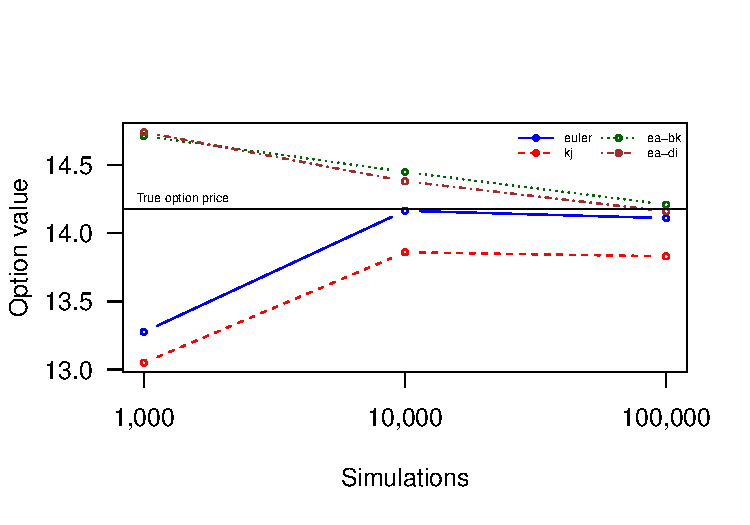
\includegraphics{thesis_files/figure-latex/modcomp1-1} 
  
  }
  
  \caption{Comparison between models 20 steps \label{modcomp1}}\label{fig:modcomp1}
  \end{figure}
  \begin{figure}
  
  {\centering 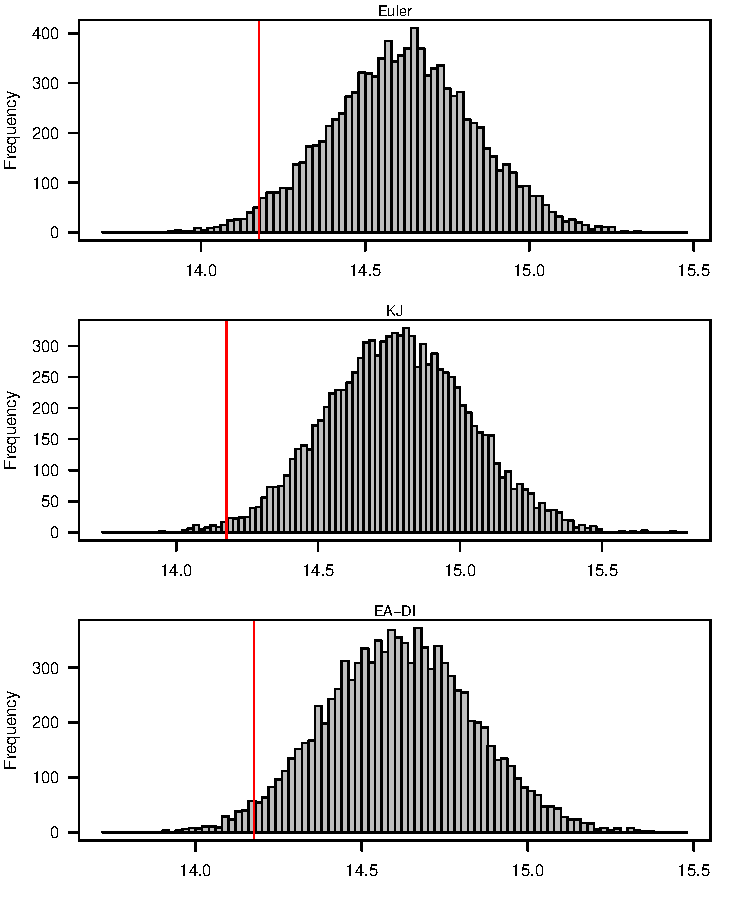
\includegraphics{thesis_files/figure-latex/results10k-1} 
  
  }
  
  \caption{Comparison between models 20 steps \label{results10k}}\label{fig:results10k}
  \end{figure}
  \begin{table}[ht]
  \centering
  \begin{tabular}{lrrrr}
    \hline 
   & Euler & KJ & EA-BK & EA-DI \\ 
    \hline 
  bias & 0.44 & 0.60 & 0.00 & 0.44 \\ 
    sd & 0.22 & 0.25 & 0.00 & 0.22 \\ 
    RMSE & 0.49 & 0.65 & 0.00 & 0.49 \\ 
    time & 1.87 & 15.59 & 0.00 & 13.27 \\ 
     \hline 
  \multicolumn{5}{l}{\scriptsize{Note: Simulations performed with 20 steps, except the EA BK}} 
  \end{tabular}
  \caption{Results} 
  \label{res}
  \end{table}
  \begin{figure}
  
  {\centering 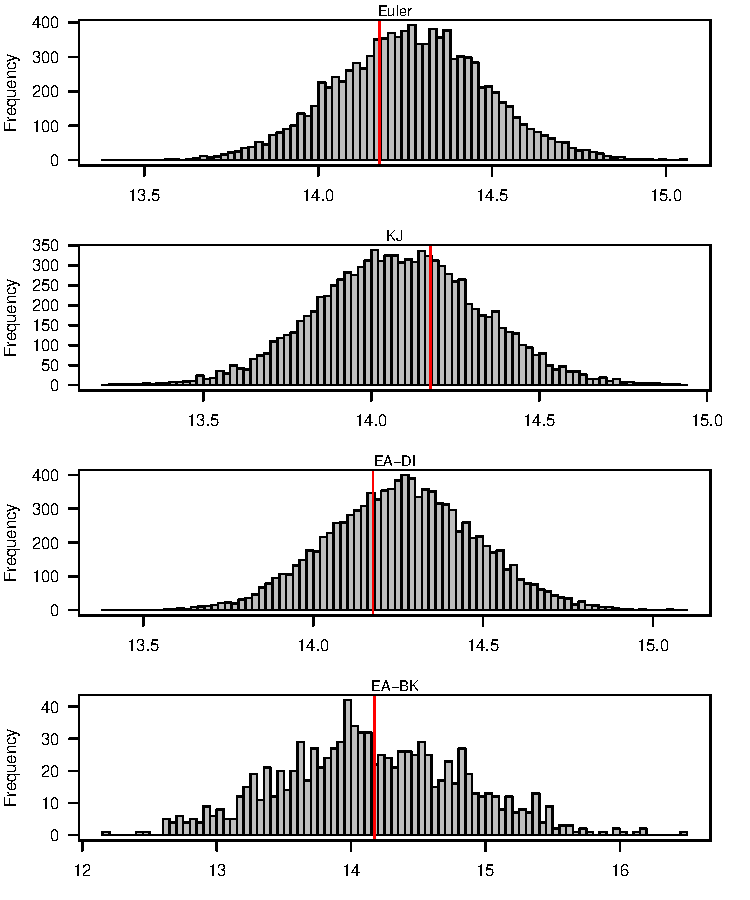
\includegraphics{thesis_files/figure-latex/results10k001-1} 
  
  }
  
  \caption{Comparison between models 100 steps \label{results10k001}}\label{fig:results10k001}
  \end{figure}
  \chapter*{Conclusion}\label{conclusion}
  \addcontentsline{toc}{chapter}{Conclusion}
  
  \chapter{Black-Scholes formula}\label{bsformula}
  
  \chapter*{References}\label{references}
  \addcontentsline{toc}{chapter}{References}
  
  \hypertarget{refs}{}
  \hypertarget{ref-heston1993closed}{}
  {[}1{]} S.L. Heston, Review of Financial Studies 6 (1993) 327--343.
  
  \hypertarget{ref-rlang}{}
  {[}2{]} R Core Team, R: A Language and Environment for Statistical
  Computing, R Foundation for Statistical Computing, Vienna, Austria,
  2017.
  
  \hypertarget{ref-nmofpack}{}
  {[}3{]} E. Schumann, Numerical Methods and Optimization in Finance
  (Nmof) Manual. Package Version 0.40-0), 2011--2016.


  % Index?

\end{document}
